%!TEX program = pdflatex
%!BIB program = bibtex
\documentclass[12pt]{article}
\usepackage{geometry}
% \geometry{left=2.0cm,right=2.0cm,top=2.5cm,bottom=2.5cm}


\usepackage{times}
\usepackage{soul}
\usepackage{url}
\usepackage[hidelinks]{hyperref}
\usepackage[utf8]{inputenc}
\usepackage[small]{caption}
\usepackage{graphicx}
\usepackage{subfigure}
\usepackage{amsmath}
\usepackage{amsthm}
\usepackage{booktabs}
\usepackage{algorithm}
\usepackage{algorithmic}
\usepackage{lipsum}
\usepackage{multirow}  % for multirow command used in the table
\usepackage{setspace}
\usepackage{ulem}  % 用于添加下划线
\urlstyle{same}

\newtheorem{example}{Example}
\newtheorem{theorem}{Theorem}


\begin{document}
\setstretch{1.5}
\linespread{1}
\title{Response to Reviewers of TCSVT-07024-2021: A Simple and Strong Baseline for Universal Targeted Attacks on Siamese Visual Tracking}
\author{Zhenbang Li, Yaya Shi, Jin Gao, Shaoru Wang, Bing Li,\\ Pengpeng Liang, Weiming Hu}
\date{}
\maketitle

\noindent Dear Editors:

When we revised the paper, we carefully considered and followed all the comments and suggestions provided by you and the reviewers. To summarize, we have made the following revisions:

(1) We adding the advantages \& limitations of the proposed method after experimental analysis and future works to the conclusion.

(2) We add 3-5 papers published in the IEEE Transactions on Circuits and Systems forVideo Technology, which are most closely related to your manuscript; b) what isdistinctive / new about your current manuscript related to these previously publishedpapers.

We hope that our revised manuscript is now appropriate for publication in IEEE Transactions on Circuits and Systems for Video Technology. Specific responses to all the comments of each reviewer are included in the rest of this document and highlighted using bold font after the comments of each reviewer for the convenience of cross-reference. To make the changes easier to identify where necessary, we also have underlined most of the revised parts in the manuscript and provide an underlined version for the convenience of second review.\\[10pt]
\indent We are looking forward to your reply.\\[10pt]
\noindent Yours sincerely,\\
\noindent Zhenbang Li, Yaya Shi, Jin Gao, Shaoru Wang, Bing Li, Pengpeng Liang, Weiming Hu
\\
\\
\\
\noindent Dr. Jin Gao (Contact author)\\
\noindent National Laboratory of Pattern Recognition (NLPR)\\
\noindent Institute of Automation, Chinese Academy of Sciences (CASIA)\\
\noindent Address: No. 95, Zhongguancun East Road, Haidian District,\\
\noindent Beijing 100190, P. R. China\\
\noindent Email: jin.gao@nlpr.ia.ac.cn

%%%%%%%%%%%%%%%%% 审稿人 1 %%%%%%%%%%%%%%%%%
\newpage
{\centering\section*{Response Letter to Reviewer \#1}}
\noindent Dear Reviewer \#1:

Thank you very much for your thorough review. Your insightful comments are very helpful for us to improve the quality of the paper. According to your comments and suggestions, we have carefully and extensively revised the manuscript. The main revised parts are highlighted by underlines in the underlined version for your convenience. You will find that all your comments and suggestions are considered and followed. We hope that our revised manuscript is now appropriate for publication in IEEE Transactions on Circuits and Systems for Video Technology.
In addition, point-to-point responses to your comments are given below and highlighted using bold font in line with your comments in order to facilitate cross-referencing.\\[10pt]
\indent We are looking forward to your reply.\\[10pt]
\noindent Yours sincerely,\\
\noindent Zhenbang Li, Yaya Shi, Jin Gao, Shaoru Wang, Bing Li, Pengpeng Liang, Weiming Hu
\\
\\
\\
\noindent Dr. Jin Gao (Contact author)\\
\noindent National Laboratory of Pattern Recognition (NLPR)\\
\noindent Institute of Automation, Chinese Academy of Sciences (CASIA)\\
\noindent Address: No. 95, Zhongguancun East Road, Haidian District,\\
\noindent Beijing 100190, P. R. China\\
\noindent Email: jin.gao@nlpr.ia.ac.cn

\newpage
\textit{This paper addresses the task of attacking Siamese network-based trackers in a simple yet effective fashion. Unlike other methods that operate in the video-specific attacking regime (which resides on network inference for generating perturbations while tracking), this method is the first to perform universal targeted attacks for Siamese trackers utilizing both the translucent perturbation and the adversarial patch together. By adding the perturbation to the template and adding the patch to the search image while performing tracking, this work fools the Siamese trackers to the fake target region and thus makes them fail in tracking the real target object. Overall, this is an interesting paper, and it is well written and organized. As it is a resubmitted manuscript, I notice that the authors have made substantial changes to the previous manuscript, which are able to appropriately respond to the comments made by the previous reviewers. Although the template perturbation and adversarial patch are both easy to observe for human eyes as the previous reviewers have pointed out, and the SSIMs for them are also lower than the video-specific attacking method, e.g., FAN \cite{FAN}, this reviewer believes that this proposed new framework can be a new configuration of adversarial attack on visual tracking for its achieved balance between the attack efficiency and the perturbation perceptibility. This new configuration will attract increasing attention from the visual tracking attack community to study on more efficient attack methods.}

\textbf{Many thanks for your positive comments on the strength of our paper and thenovelty of the proposed attack method.}

%%%% 问题 1.1 %%%%
\textit{In addition, I suggest the authors add more experiments to demonstrate the practicability of the attack method when the ground truth box information is missing in the training data. The experimental results show that it is effective to use the predicted boxes instead of ground truth boxes for training perturbations.}

\textbf{This question needs to be discussed with Jin Gao.}

%%%% 问题 1.2 %%%%
\textit{A small question is that it will be better if the authors can provide some pseudo code for the untargeted attack and targeted attack processes in addition to the training process. This will facilitate the understanding of the attacking process while performing tracking.}

\begin{algorithm}[tb]
    \caption{Attack Process}
    \label{alg:algorithm_attack}
    \textbf{Input}: Imperceptible perturbation $\delta$, adversarial patch $p$, Siamese tracker $f$, video $V=\{I_i\}_1^T$, $b^{gt}_1$ is the position of the real target in the first frame. $B^{fake}=\{b^{fake}_i\}_1^{T}$ is the trajectory we hope the tracker to output.\\
    \textbf{Output}: $B^{pred}=\{b^{pred}_i\}_1^{T}$
    \begin{algorithmic}[1] %[1] enables line numbers
      \STATE Generate the clean template image $\textbf{z}_1$ according to $I_1$ and $b^{gt}_1$.
      \STATE Generate the perturbed template image $\tilde{\textbf z}_1=\textbf z_1+\delta$.
      \STATE Let $i = 2$.
    \WHILE{$i \le T$}
    \STATE Generate clean search image $\textbf{x}_i$ according to $I_i$ and $b^{pred}_{i-1}$.
    \STATE $b^{fake}_i=\{x_{0_i}, y_{0_i}, x_{1_i}, y_{1_i}\}$
    \STATE Generate the perturbed searach image $\tilde{\textbf x} = A_{\text{add}}(\textbf x, p_k, \{x_0, y_0, x_1, y_1\}).$
    \STATE $\textbf{C, R, Q} = f(\tilde {\textbf x}_i, \tilde{\textbf z}_1).$
    \STATE Generate the predicted bounding box $b^{pred}_t$ according to $\textbf{C, R, Q}$.
    \STATE $i = i + 1.$
    \ENDWHILE
    \STATE \textbf{return} $\delta_N, p_N.$
    \end{algorithmic}
  \end{algorithm}

\textbf{Both the targeted attack and untargeted attack process follow the same steps as shown in Alg. \ref{alg:algorithm_attack}. The difference between the target attack and the untargeted attack is the evaluation. For the targeted attack, we compare the AO between $B^{pred}=\{b^{pred}_i\}_1^{T}$ and $B^{fake}=\{b^{fake}_i\}_1^{T}$. For the untargeted attack, we compare the AO between $B^{pred}=\{b^{pred}_i\}_1^{T}$ and $B^{gt}=\{b^{gt}_i\}_1^{T}$.}

%%%% 问题 1.3 %%%%
\textit{In addition, the font size in Fig. 9 is too small to read on my computer, which needs to be improved.}

\newgeometry{left=1cm,right=1cm,top=1cm,bottom=1cm}

\begin{figure*}[t!]
  \renewcommand\thefigure{9}
  \begin{center}
    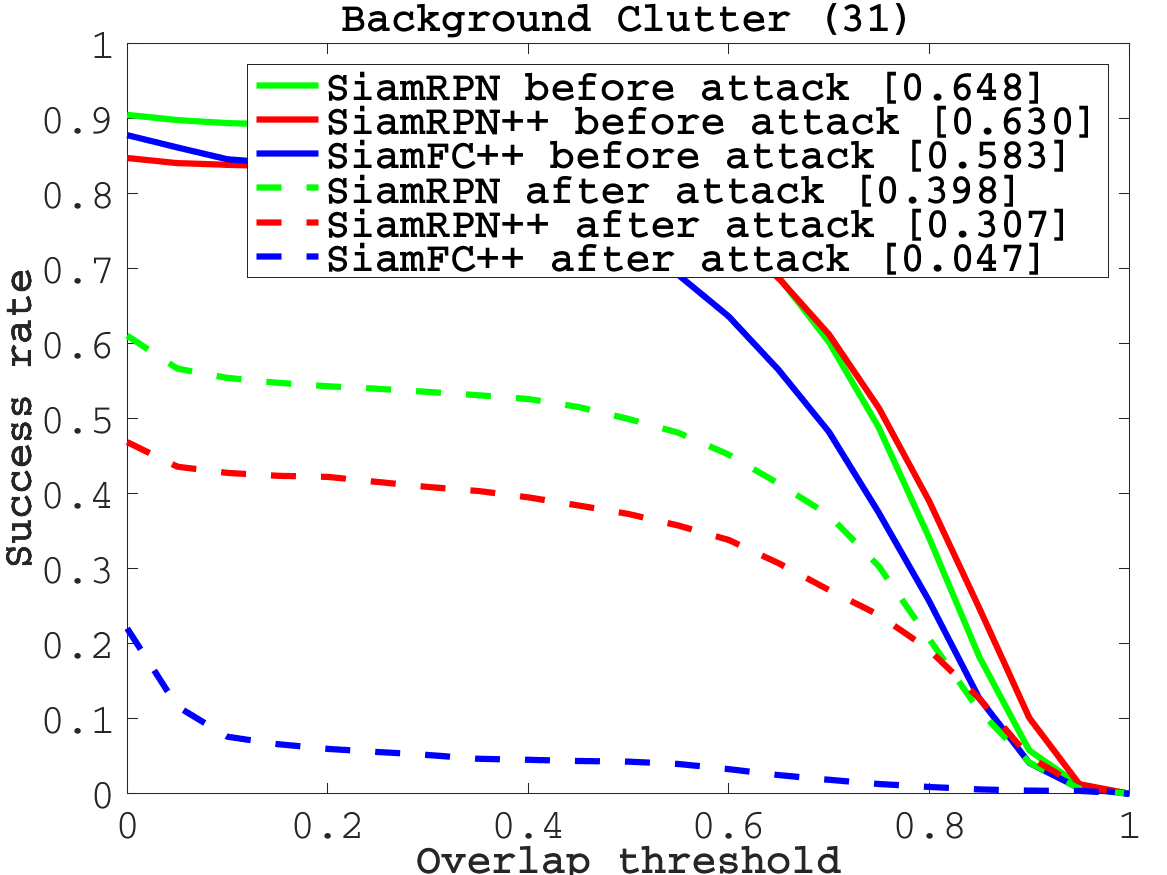
\includegraphics[width=0.32\textwidth]{images_imperceptible/OTB2015/success_plot_OPE_OTB100_BC.png}
    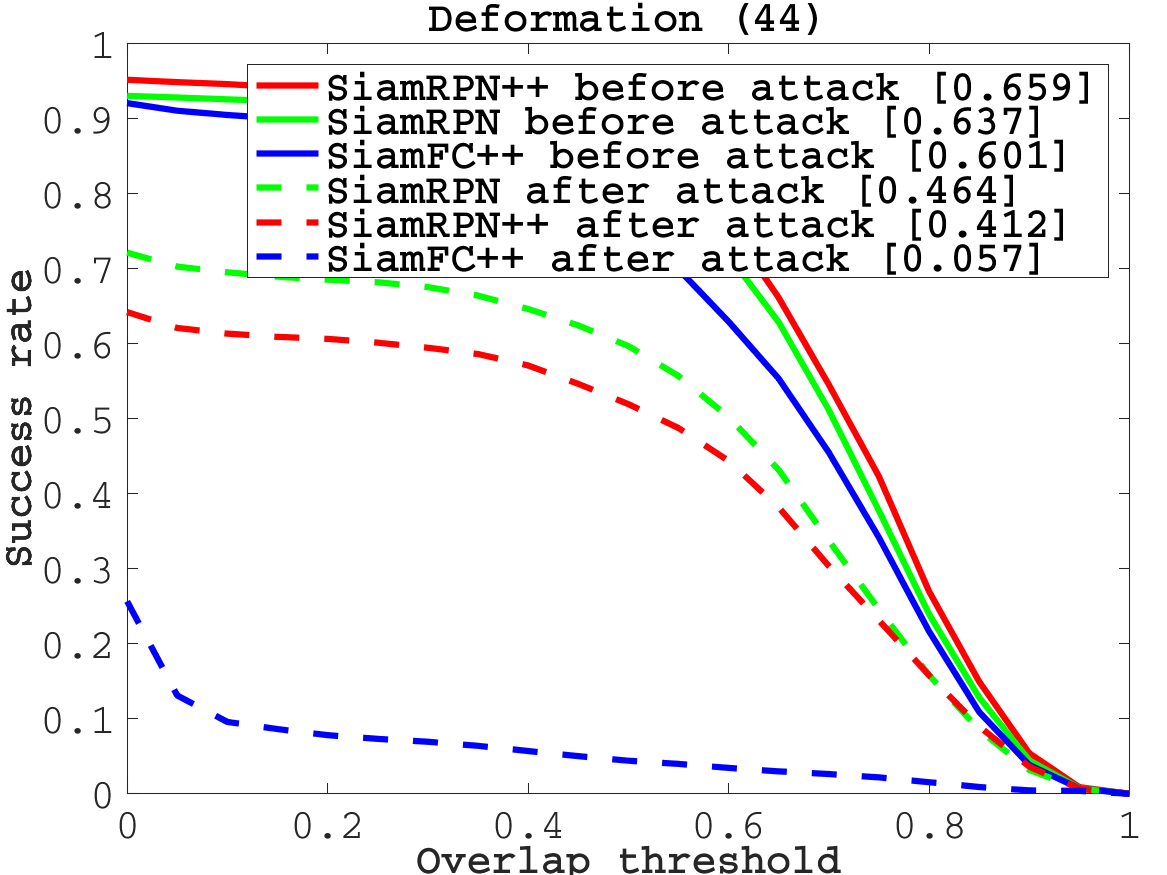
\includegraphics[width=0.32\textwidth]{images_imperceptible/OTB2015/success_plot_OPE_OTB100_DEF.png}
    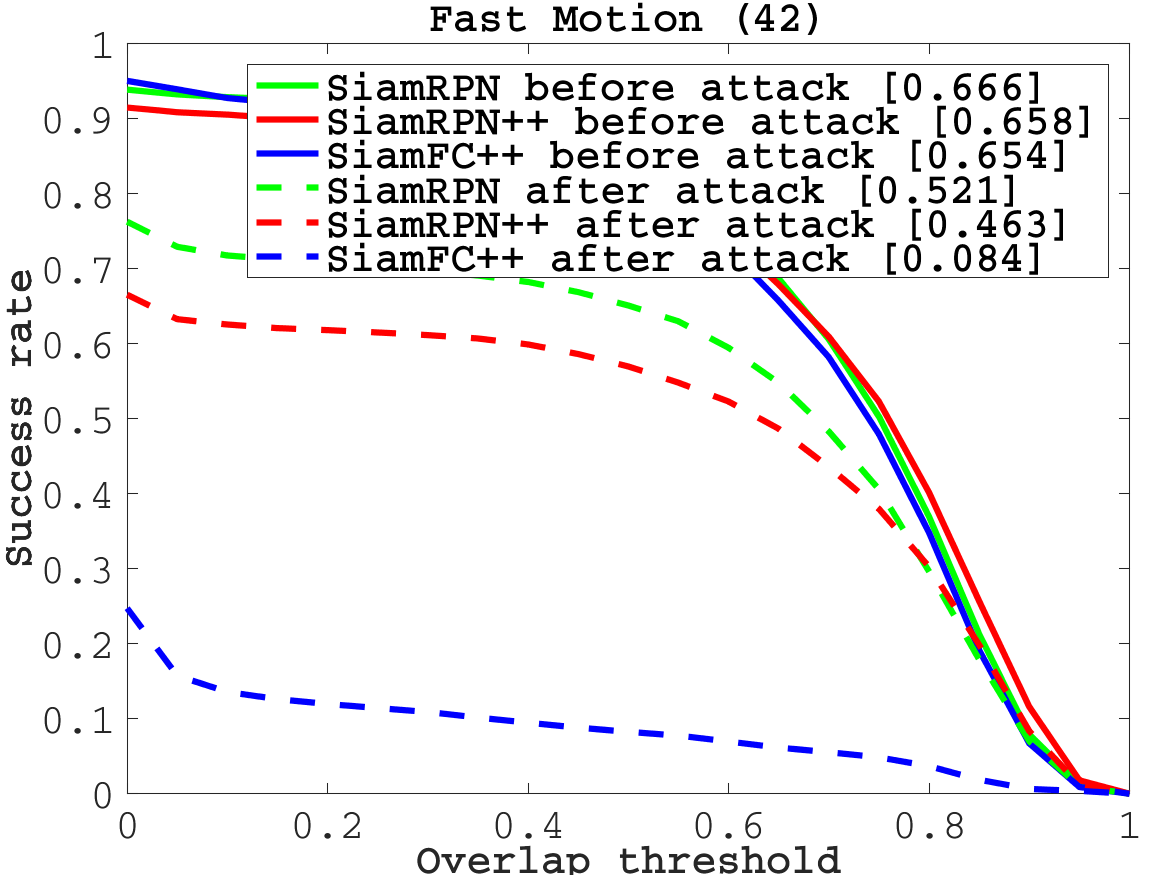
\includegraphics[width=0.32\textwidth]{images_imperceptible/OTB2015/success_plot_OPE_OTB100_FM.png}
    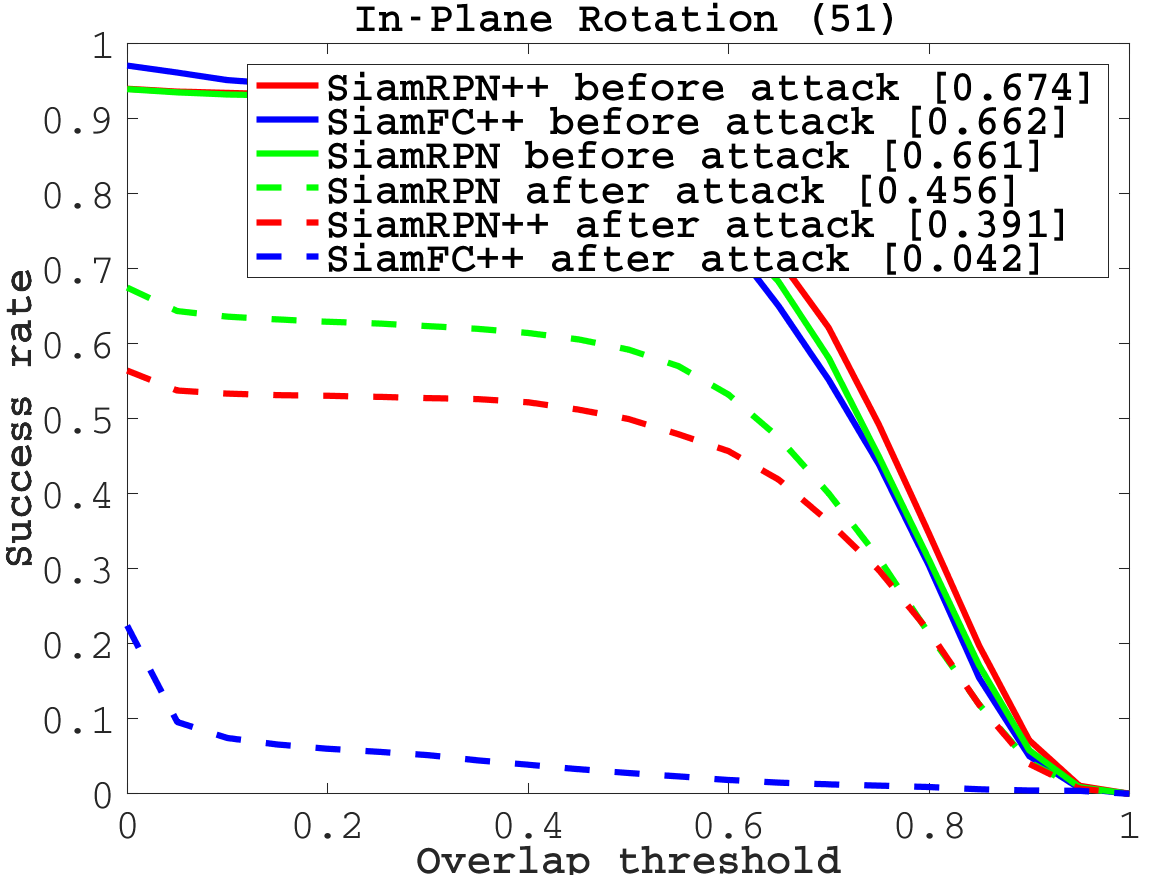
\includegraphics[width=0.32\textwidth]{images_imperceptible/OTB2015/success_plot_OPE_OTB100_IPR.png}
    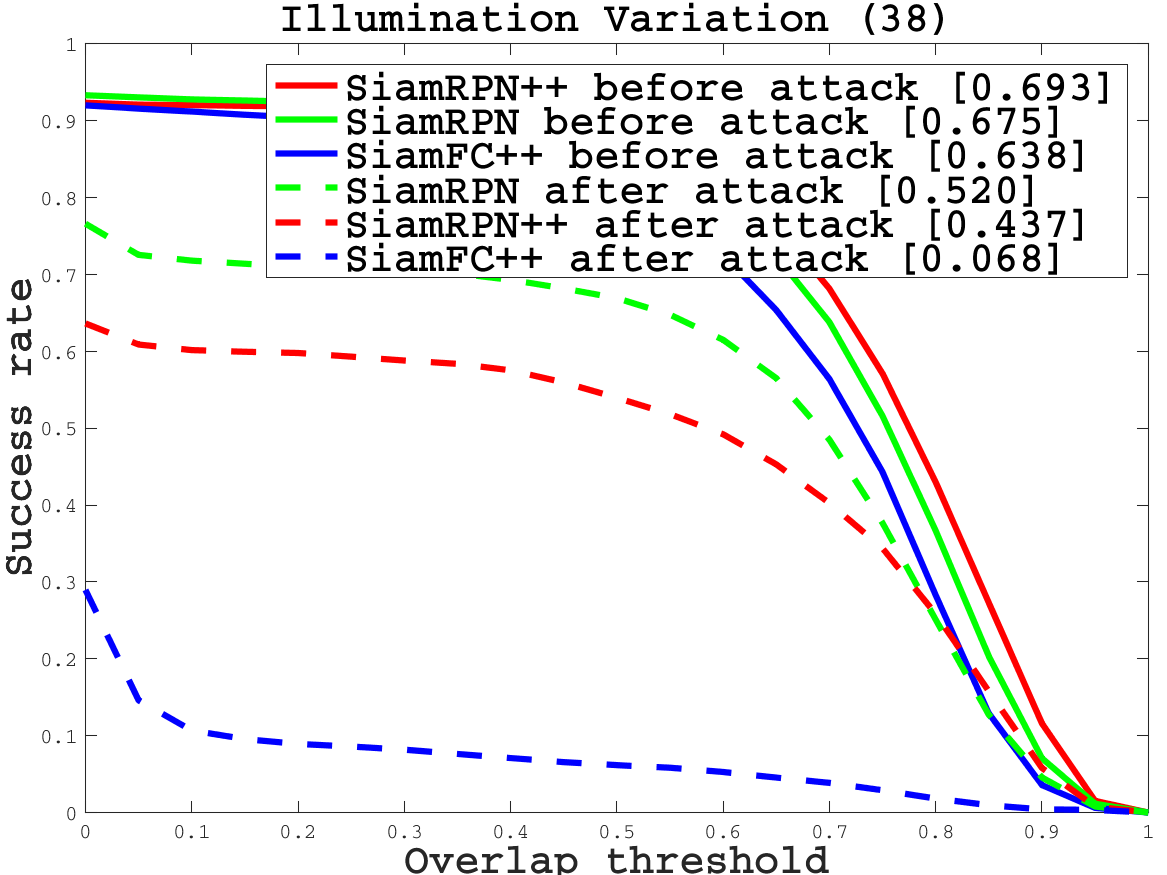
\includegraphics[width=0.32\textwidth]{images_imperceptible/OTB2015/success_plot_OPE_OTB100_IV.png}
    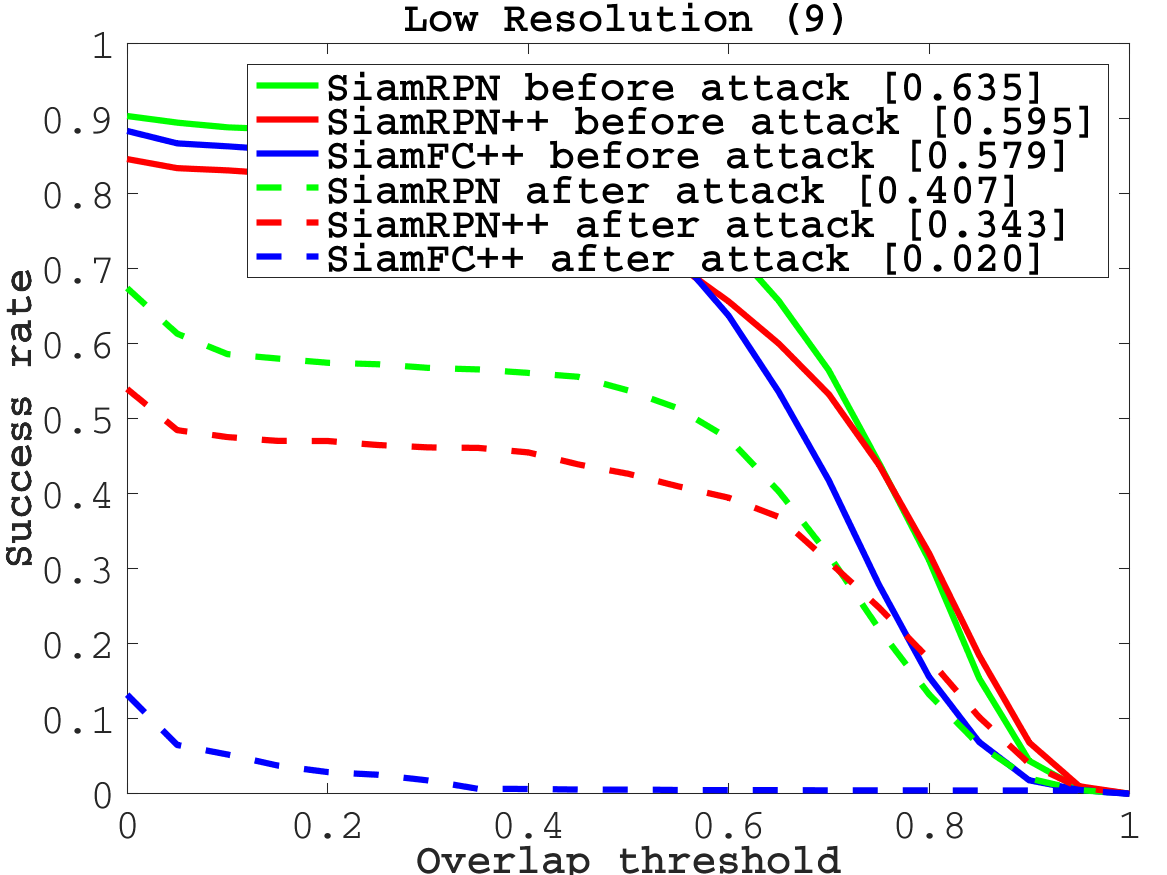
\includegraphics[width=0.32\textwidth]{images_imperceptible/OTB2015/success_plot_OPE_OTB100_LR.png}
    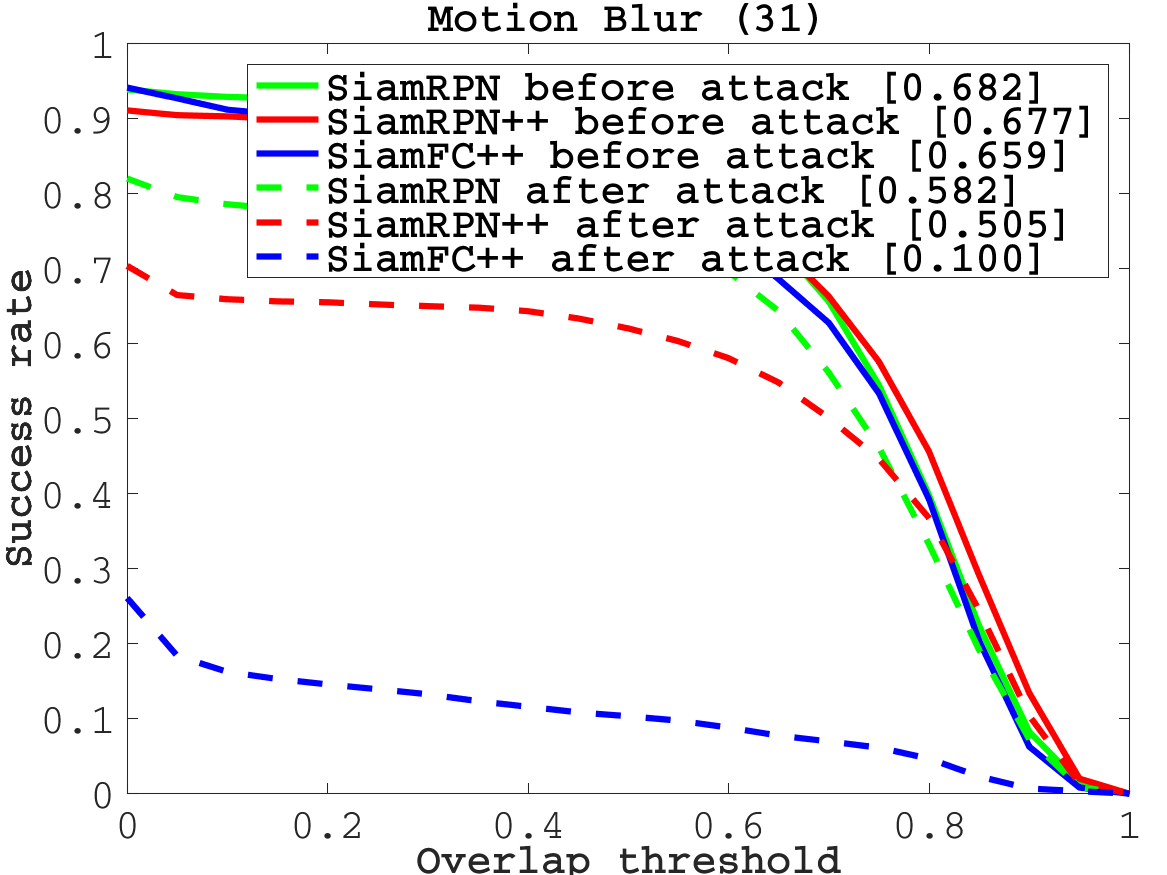
\includegraphics[width=0.32\textwidth]{images_imperceptible/OTB2015/success_plot_OPE_OTB100_MB.png}
    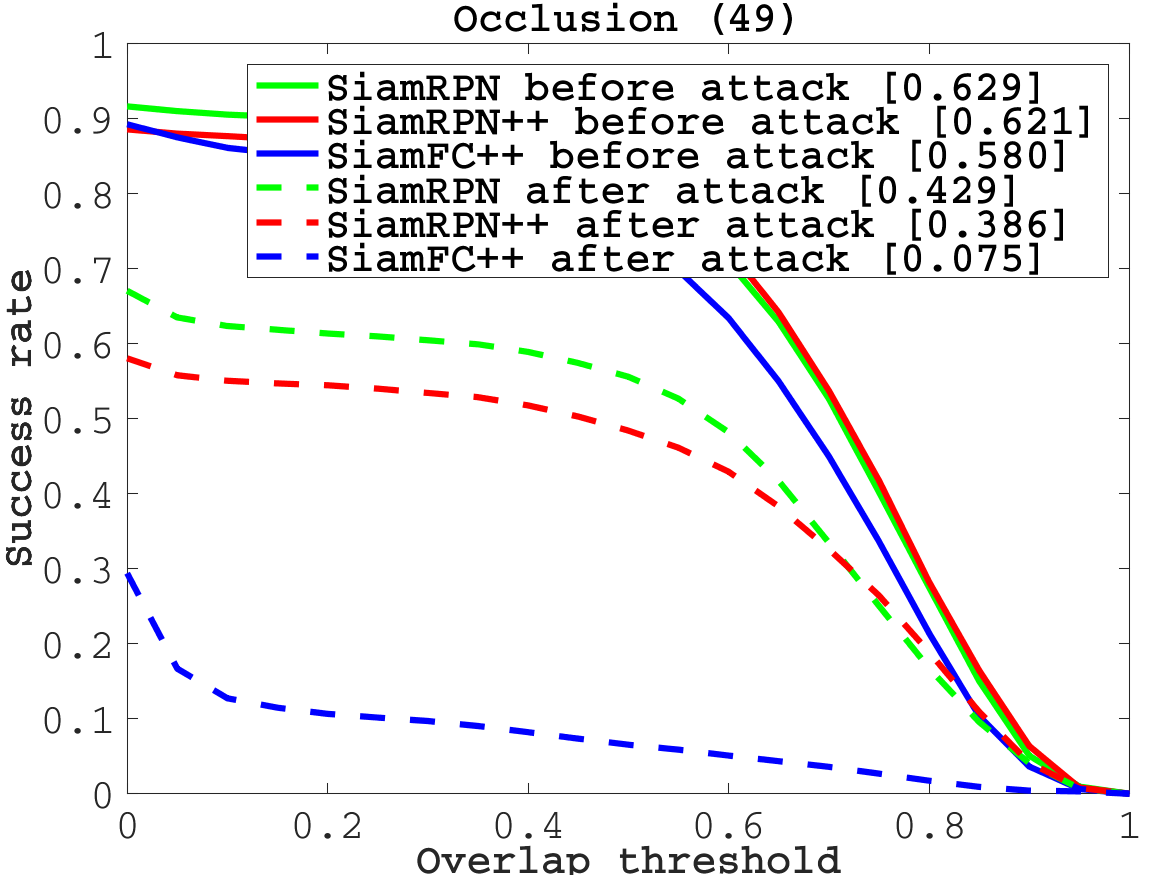
\includegraphics[width=0.32\textwidth]{images_imperceptible/OTB2015/success_plot_OPE_OTB100_OCC.png}
    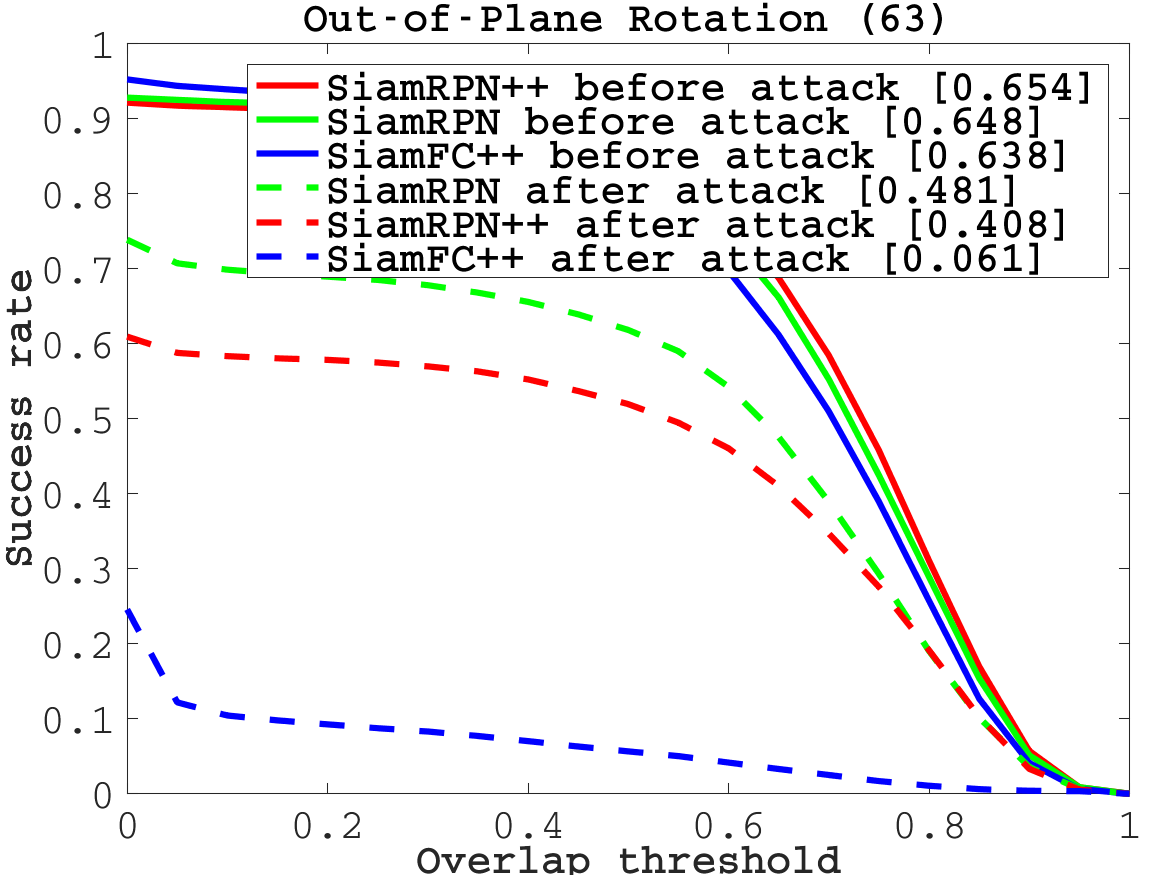
\includegraphics[width=0.32\textwidth]{images_imperceptible/OTB2015/success_plot_OPE_OTB100_OPR.png}
    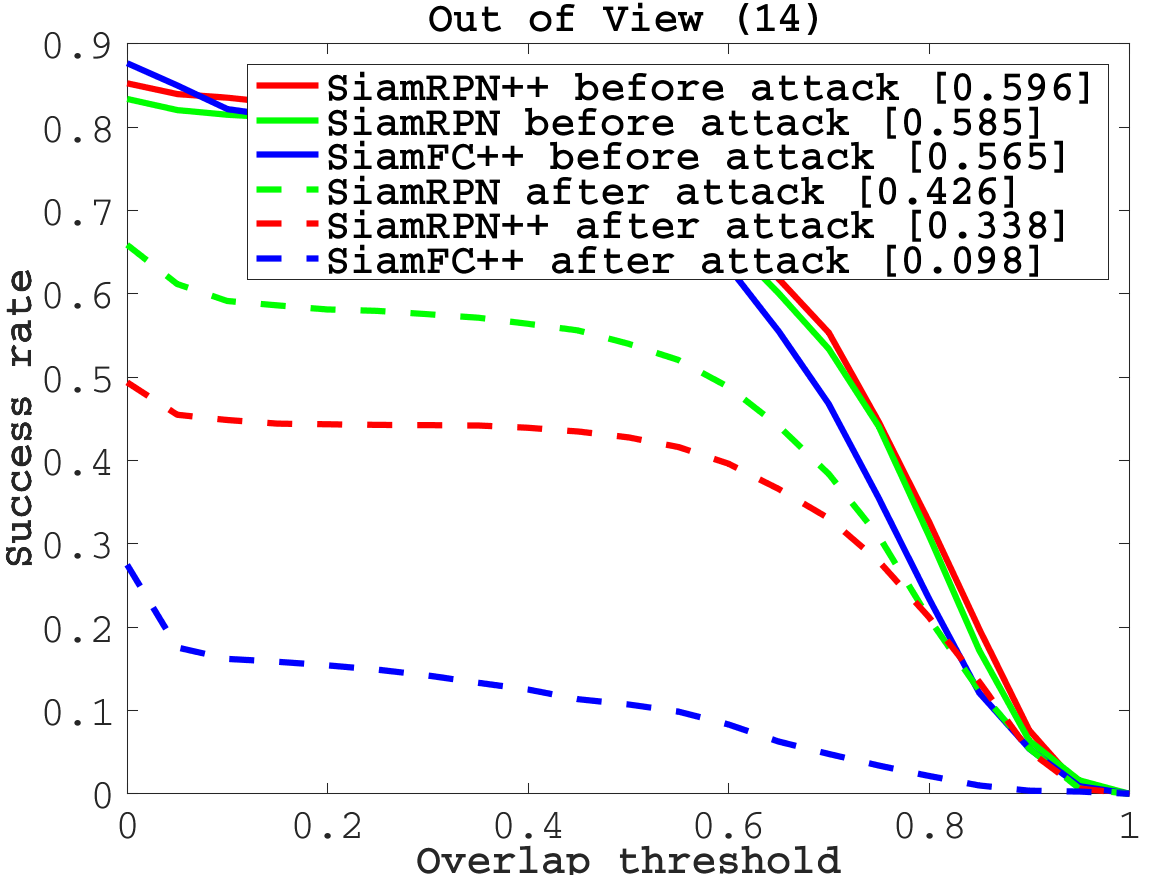
\includegraphics[width=0.32\textwidth]{images_imperceptible/OTB2015/success_plot_OPE_OTB100_OV.png}
    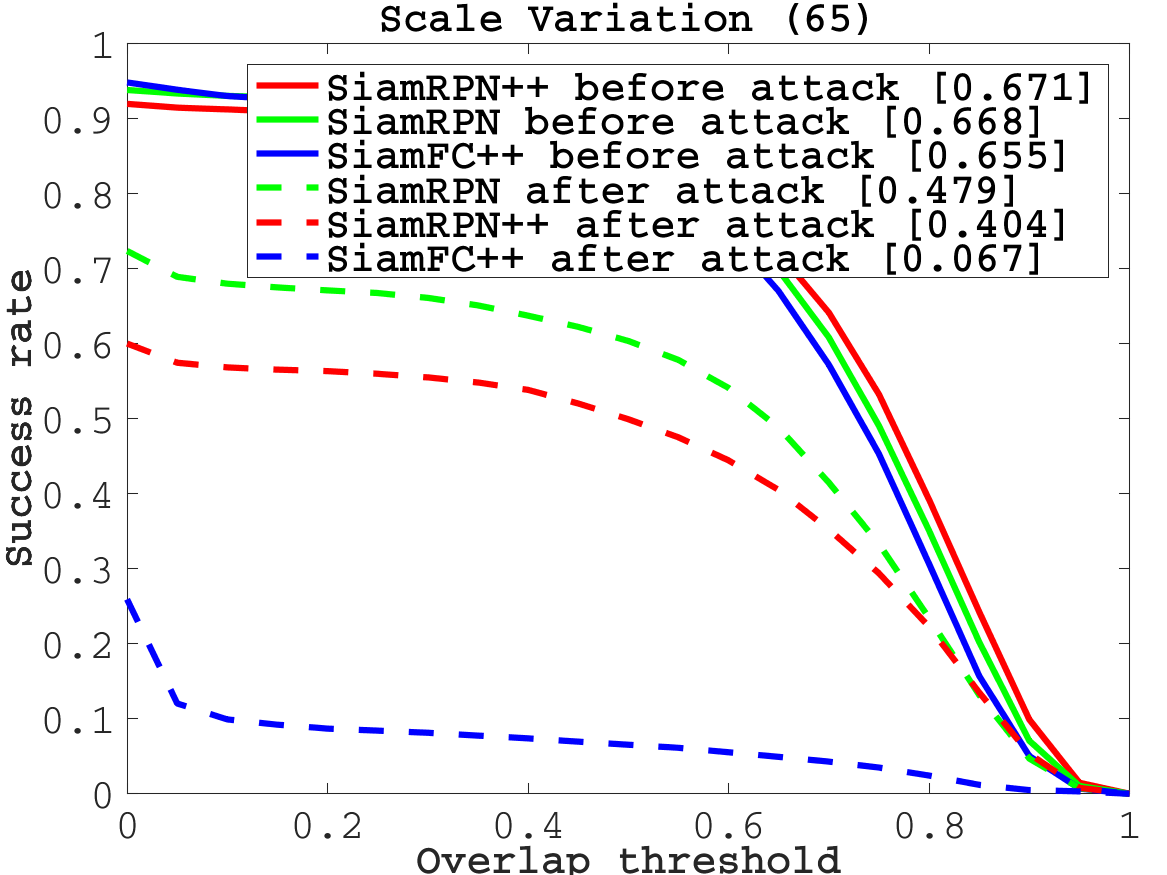
\includegraphics[width=0.32\textwidth]{images_imperceptible/OTB2015/success_plot_OPE_OTB100_SV.png}
  \end{center}
      \caption{Untargeted attack results of the different trackers under the 11 attributes: out-of-view (OV), occlusion (OCC), illumination variation (IV), out-of-plane rotation (OPR), scale variation (SV),deformation (DEF), low resolution (LR), fast motion (FM), background clutters (BC), motion blur (MB), and in-plane rotation (IPR). The results show good transferability of our attacks to different tracking architectures, even if the generated perturbations are applied to anchor-based trackers.}
  \label{fig:attr}
\end{figure*}

\restoregeometry

%%%% 问题 1.4 %%%%
\textit{Also, some recent papers are valued to be referred (2020-2021), to ehahnce the quality.}

\textbf{...}

%%%%%%%%%%%%%%%%% 审稿人 2 %%%%%%%%%%%%%%%%%
\newpage
{\centering\section*{Response Letter to Reviewer \#2}}
\noindent Dear Reviewer \#2:

Thank you very much for your thorough review. Your insightful comments are very helpful for us to improve the quality of the paper. According to your comments and suggestions, we have carefully and extensively revised the manuscript. The main revised parts are highlighted by underlines in the underlined version for your convenience. You will find that all your comments and suggestions are considered and followed. We hope that our revised manuscript is now appropriate for publication in IEEE Transactions on Circuits and Systems for Video Technology.
In addition, point-to-point responses to your comments are given below and highlighted using bold font in line with your comments in order to facilitate cross-referencing.\\[10pt]
\indent We are looking forward to your reply.\\[10pt]
\noindent Yours sincerely,\\
\noindent Zhenbang Li, Yaya Shi, Jin Gao, Shaoru Wang, Bing Li, Pengpeng Liang, Weiming Hu
\\
\\
\\
\noindent Dr. Jin Gao (Contact author)\\
\noindent National Laboratory of Pattern Recognition (NLPR)\\
\noindent Institute of Automation, Chinese Academy of Sciences (CASIA)\\
\noindent Address: No. 95, Zhongguancun East Road, Haidian District,\\
\noindent Beijing 100190, P. R. China\\
\noindent Email: jin.gao@nlpr.ia.ac.cn

\newpage
\textit{In this paper, the authors train a universal adversarial patch to add on both template and search regions of a Siamese based tracker to deteriorate its original performance. The proposed perturbations are video-agnostic, leading to a low computational cost during attack. The experiment validations show that the proposed method achieves favorable attack results on OTB2015, GOT-10k, LaSOT, UAV123, VOT2016, VOT2018 and VOT2019. In addition, the generated perturbations transfer well on other Siamese trackers as well. The idea of this paper is interesting and the experiments are thorough.}

\textbf{Many thanks for your positive comments on the strength of our paper and the novelty of the proposed attack method.}

%%%% 问题 2.1 %%%%
\textit{However, there are some concerns over the implementation, performance and writing. 1. The authors state that training with Ep. 4 leads to an obvious patch on the images while using Eq.5 into the training process results in a less obvious patch. The reviewer considers that giving a constraint (e.g. $l_inf$) on the $p_x$ in Eq.4 can make the perturbation imperceptible intuitively. Please give more analysis on this setting.}

\textbf{Sorry that we did not clarify the meaning of paste. If we paste the perturbation, we means we use a patch to replace the original image, which means the patch and the original image is discrete (even if we give a constraint).}

\textit{Besides, the reviewer hopes to know the reason why give an extra perturbation on the template region. The perturbations on template and search regions look similar, while the authors say that they are different. Please state the difference between the patch application operator on search examples and the operator on template examples.}

\textbf{The operator $A_{\text{add}}(\textbf{x}, p_\textbf{x}, b^{fake}_{\textbf{x}})$ and $\textbf{z} + \delta_\textbf{z})$ is similar. The only difference is that, $A_{\text{add}}$ means add the perterbation to a specific region because the patch size is less than the image, while $+$ means add the perturbation to the full image because the size is the same.}

\textit{In addition, the denotations of $A_paste$ in Eq.4 and $A_add$ in Eq.5 seem like the same one.}

\textbf{Sorry that we make the wrong citation and not clarify the meaning of add and paste. If we paste the perturbation, we means we use a patch to replace the original image, which means the patch and the original image is discrete (even if we give a constraint). The final pixel value is changed from the original value to a new value. If we add a patch onto the image, the final pixel value is the original value plus a new value.}


%%%% 问题 2.2 %%%%
\textit{2. I agree with reviewer 3, the ground truth boxes are inaccessible to trackers during the inference. It seems that the authors use the ground truth boxes to generate the fake trajectory in lines 51-57 on page 7. Please clarify it.}

\textbf{We generate new trajectory without the test GT: we let the fake box run straight to border of the image, speed and derection is random.}

\begin{table}[t]
  \centering
  \begin{tabular}{@{}lllll@{}}
  \toprule
         & \multicolumn{2}{l}{Untargeted Attack} & \multicolumn{2}{l}{Targeted Attack} \\
         & AO                & SR                & AO               & SR               \\ \midrule
  track2 & 0.1747            & 0.1442            & 0.8448           & 0.8972           \\ \bottomrule        
  \end{tabular}
  \end{table}

%%%% 问题 2.3 %%%%
\textit{3. For the experiments, the authors should conduct the ablation study on only adding perturbations on the template images or the search regions to show the impact of $p$ and $\delta$.}

\textbf{Thanks for your advice and we have conducted the ablation study on only adding perturbations on the template images or the search regions to show the impact of $p$ and $\delta$. As we can see, only use one of them is not useful, because they are trained together.}

\begin{table}[]
  \centering
  \begin{tabular}{@{}lllll@{}}
  \toprule
                & \multicolumn{2}{l}{Untargeted Attack} & \multicolumn{2}{l}{Targeted Attack} \\
                & AO                & SR                & AO               & SR               \\ \midrule
  Only Template & 0.5097            & 0.5669            & 0.1555           & 0.1064           \\
  Only Search   & 0.7137            & 0.8414            & 0.1599           & 0.1320           \\ \bottomrule
  \end{tabular}
\end{table}

%%%% 问题 2.4 %%%%
\textit{4. As reviewer 1 and reviewer 2 say, the perturbations added to template regions and research regions are not imperceptible, which may be helpful to misguide the tracker. The reviewer considers that adding a similar random pattern on the template and search regions to further illustrate the effectiveness of the proposed method.}

\textbf{Need to be discussed with (at least conformed by) JinGao: What is the similar random pattern ?}

%%%% 问题 2.5 %%%%
\textit{
5. There are some minor problems, grammar errors and typos in this paper. The reviewer hopes the authors polish this paper again. 
- On page 2, ‘1016’ -> ‘2016’ in line 56. There is a same one in line 47 on page 6.
- The denotation of $B_x^fake$ in Eq.4 is not clear enough, even though it can be inferred by the later part.
- On page 4, ‘imperceptible’ -> ‘imperceptibly’ in line 57.
- The reinitialization of VOT-toolkit should be mentioned in the part of ‘experimental setup’.
- On page 7, ‘.(see Table I)’ is a typo.
}

\textbf{Thanks for your advice and we have changed this errors.}

%%%%%%%%%%%%%%%%% 审稿人 3 %%%%%%%%%%%%%%%%%
\clearpage
\newpage
{\centering\section*{Response Letter to Reviewer \#3}}
\noindent Dear Reviewer \#3:

Thank you very much for your thorough review. Your insightful comments are very helpful for us to improve the quality of the paper. According to your comments and suggestions, we have carefully and extensively revised the manuscript. The main revised parts are highlighted by underlines in the underlined version for your convenience. You will find that all your comments and suggestions are considered and followed. We hope that our revised manuscript is now appropriate for publication in IEEE Transactions on Circuits and Systems for Video Technology.
In addition, point-to-point responses to your comments are given below and highlighted using bold font in line with your comments in order to facilitate cross-referencing.\\[10pt]
\indent We are looking forward to your reply.\\[10pt]
\noindent Yours sincerely,\\
\noindent Zhenbang Li, Yaya Shi, Jin Gao, Shaoru Wang, Bing Li, Pengpeng Liang, Weiming Hu
\\
\\
\\
\noindent Dr. Jin Gao (Contact author)\\
\noindent National Laboratory of Pattern Recognition (NLPR)\\
\noindent Institute of Automation, Chinese Academy of Sciences (CASIA)\\
\noindent Address: No. 95, Zhongguancun East Road, Haidian District,\\
\noindent Beijing 100190, P. R. China\\
\noindent Email: jin.gao@nlpr.ia.ac.cn

\newpage

%%%% 问题 3.1 %%%%
\textit{This paper employs the universal perturbation attacks on Siamese visual trackers. There are still the following concerns about the proposed method. 1. As stated in the paper, the proposed method " does not require gradient optimization or network inference". However, this is a double-edged sword since it resulted in suspicious attacks. Prior works commonly train a network to prevent not only suspicious attacks but also modifying every pixel. I think it's a major problem with this work. I suggest considering a proper strategy to remove/reduce it.}

\textbf{Thanks for your advices. Our patch is obvious (SSIM=0.56). We think the main reason is that we have to learn useful information in such small regions 64*64 as a fake target. While the information of the real target is not changed. So it may be top heat map on the real object, so the network will work hard to create a fake target, which lead to high perturbation values. But, if we can break the target information, it will be easy to attack.
Our solution is attack the whole image. Y channel, CbCr channel. 
}

%%%% 问题 3.2 %%%%
\textit{2. The proposed method and offline training phase should be explained more clearly. For instance, the termination of offline training or offline optimization is missed affecting perturbation values.}

\textbf{...}

\textit{3. The descriptions of figures and tables are not self-explanatory.}

\textbf{...}

\textit{4. I suggest adding the advantages \& limitations of the proposed method after experimental analysis and future works to the conclusion.}

\textbf{
Advantages:
  (1) Because our video-agnostic feature, we are fast, no need to network interferes or gradient calculation.
  (2) Good transferability to other trackers.
Disadvantages:
  (1) Physical attack. We are the digital attack, which means ... Physical attack is ... The advantage of it is ... Our work assumes a threat model in which the adversary can feed data directly into the machine learning classifier. This is not always the case for systems operating in the physical world, for example those which are using signals from cameras and other sensors as input.
  % 这不就是 ICCV2019 的工作吗?它们也通用?好像是。EOT是通用的吗?
  (2) Not imperceptible.
  % 防御?
Future work:
  (1) We need to do the physical attack.
  (2) We need to be imperceptible.
  % 使用同一个扰动同时攻击多个视觉任务,包括图像分类,检测,视频目标跟踪和分割。
  Use a single perturbation to attack multi vision task, including image classification, object detection and video object tracking/segementation.
  % 以更小的扰动取得更高的攻击效果。(呼应缺点之:扰动大)
  Use more imperceptible perturbations to achieve high attack performance.
  % 本文所提出的对抗性信息被添加在数字图像上,从而影响跟踪器的跟踪效果。然而所提出的对抗性信息难以用于执行孪生跟踪器的物理攻击,即将对抗扰动打印出来添加到物理世界的真实目标上,从而影响孪生跟踪系统的性能。因为对抗扰动的打印过程可能改变扰动的值,且相机传感器可能无法感知较小的扰动。可能的解决方案是借助EOT生成针对相机距离和角度具有鲁棒性的物理扰动,使得在各种成像条件下,跟踪系统都无法对带有对抗性信息的真实目标进行正确跟踪。
  % 通过 *** 方式(比如,借助 *** 信息)实现物理攻击。
}

\textit{5. Some of the experiments require more explanations. For example, transferability has been investigated by different backbones \& architectures. It's needed to mention these experiments are with/without the training phase or not.}

\textbf{Thanks for point out this. These experiments do not need the training phase.}

\textit{6. In experiments, I suggest considering two scenarios of different directions and trajectories.}

\textbf{We generate new trajectory without the test GT: we let the fake box run straight to border of the image, speed and derection is random.}

\textit{7. There are still some typo and grammar mistakes in the paper.}

\textbf{...}

\textit{8. Missing key ref : "Deep Learning for Visual Tracking: A Comprehensive Survey," in IEEE Transactions on Intelligent Transportation Systems, 2021.}

%%%%%%%%%%%%%%%%% 审稿人 4 %%%%%%%%%%%%%%%%%
\clearpage
\newpage
{\centering\section*{Response Letter to Reviewer \#4}}
\noindent Dear Reviewer \#4:

Thank you very much for your thorough review. Your insightful comments are very helpful for us to improve the quality of the paper. According to your comments and suggestions, we have carefully and extensively revised the manuscript. The main revised parts are highlighted by underlines in the underlined version for your convenience. You will find that all your comments and suggestions are considered and followed. We hope that our revised manuscript is now appropriate for publication in IEEE Transactions on Circuits and Systems for Video Technology.
In addition, point-to-point responses to your comments are given below and highlighted using bold font in line with your comments in order to facilitate cross-referencing.\\[10pt]
\indent We are looking forward to your reply.\\[10pt]
\noindent Yours sincerely,\\
\noindent Zhenbang Li, Yaya Shi, Jin Gao, Shaoru Wang, Bing Li, Pengpeng Liang, Weiming Hu
\\
\\
\\
\noindent Dr. Jin Gao (Contact author)\\
\noindent National Laboratory of Pattern Recognition (NLPR)\\
\noindent Institute of Automation, Chinese Academy of Sciences (CASIA)\\
\noindent Address: No. 95, Zhongguancun East Road, Haidian District,\\
\noindent Beijing 100190, P. R. China\\
\noindent Email: jin.gao@nlpr.ia.ac.cn

\newpage
\textit{This paper proposes a universal targeted attacks method on Siamese visual tracking task. It seems that the method is feasible and somewhat novel.}

\textbf{...}

\textit{My major concern is that the writing and organization need to be carefully modified and optimized. Besides, 1. Authors are focused on the anchor-free tracker in the experiments, but the anchor-free Siamese trackers are not well mentioned. I suggest the authors to include the discussion of state-of-the-art of other similar approaches (e.g., FCOT, SiamCAR, OCEAN, et. al.).}

\textbf{...}

\textit{2. The model is trained based on Eq.11 and Eq.12. It is not clear why the sign function is introduced. It is also suggested to describe the derivation of these two equations in detail.}

\textbf{The sign function is the FGSM method.}

\textit{3. The format of all the Tables is suggested to be unified.}

\textbf{...}

\textit{
4. There are many typos in the paper, including but not limited to the following errors:
(a) In the third line below Eq.7, $A_{a}dd$ should be $A_{add}$.
(b) In page 2, difference datasets GOT-10K[12], LaSOT \cite{LaSOT} cite the same reference.
(c) In page 3, Subsection A of Section 3, “to get an template image” should be “to get a template image”.
}

\textbf{...}

\normalem
\bibliographystyle{IEEEtran}
\bibliography{ref.bib}

\end{document}

